\chapter{Implementation}\label{chapter:implementation}

The implementation chapter will provide specific information about the CASA system implemented for the thesis. It will give more attention to the algorithms used for different parts of the architecture and their input parameters. The main goal of the system was to separate monophonic piano music from the background noise by finding an ideal binary mask for the cochleagram. The follow-up experiments will be described later in chapter \ref{chapter:experiments}.\\

It should also be noted, that the implemented system is rather simple, thus it should not be expected to observe source separation of too high quality. The implemented model serves only as an example of a CASA system and is not aiming to separate the sources using the most modern and sophisticated algorithms and approaches.\\

The system is implemented in Python with the help of \textit{numpy} \cite{Harris2020}, \textit{scipy} \cite{Virtanen2020}, \textit{statsmodels} \cite{Seabold2010}, \textit{matplotlib} \cite{Hunter2007} and \textit{brian2hears} \cite{Stimberg2019brian2hears} packages. \textit{skimage} \cite{VanDerWalt2014} and \textit{brian2} \cite{Stimberg2019brian2} were used as supporting ones. The main Python scripts contain functions for different parts of the resulting architecture, and then an example of their usage along with the experiments overview is given in the supporting Jupyter notebooks (see the structure of the attached medium for more information).

\section{Cochleagram}

The cochleagram described in chapter \ref{subsection:casa_peripheral_analysis} was implemented with the help of \textit{brian2hears}~\cite{Stimberg2019brian2hears} package. At the beginning, an array of center frequencies was computed using the ERB-rate scale defined in chapter \ref{section:math_concepts}. In the main example notebook, there were 128 center frequencies uniformly distributed on it between the values of the lowest and the highest fundamental frequencies on the standard piano keyboard (containing 88 keys) -- from $27.5$\,Hz (note $A_0$) to $4.186$\,kHz (note $C_8$).\\

As a next step, a gammatone filterbank was used to split the input into 128 corresponding frequency channels. The filters were implemented as cascades of four IIR filters of order~2 (which corresponds to single gammatone filters of order~4 \cite{Stimberg2019brian2hears}). The approximate impulse response was similar to the one defined in equation \ref{equation:gammatone_impulse_response}:
\begin{equation}
	g_{f_c}(t) = t^3\,e^{-2\pi{}bERB(f_c)t}\,\cos(2\pi{}f_c{}t)
\end{equation}
where $b=1.019$ and the ERB function was the same as in equation \ref{equation:ERB_1990} for frequency in Hertz. Finally, a unit-step function was applied to the output along with a cubic root function that helped to better emphasize low amplitudes in the cochleagram. The resulting cochleagrams for C-major and A-major scales are shown on figure \ref{img:cochleagram_example}.\\

\begin{figure}[t]
	\centering
	\begin{subfigure}{0.5\textwidth}
		\centering
		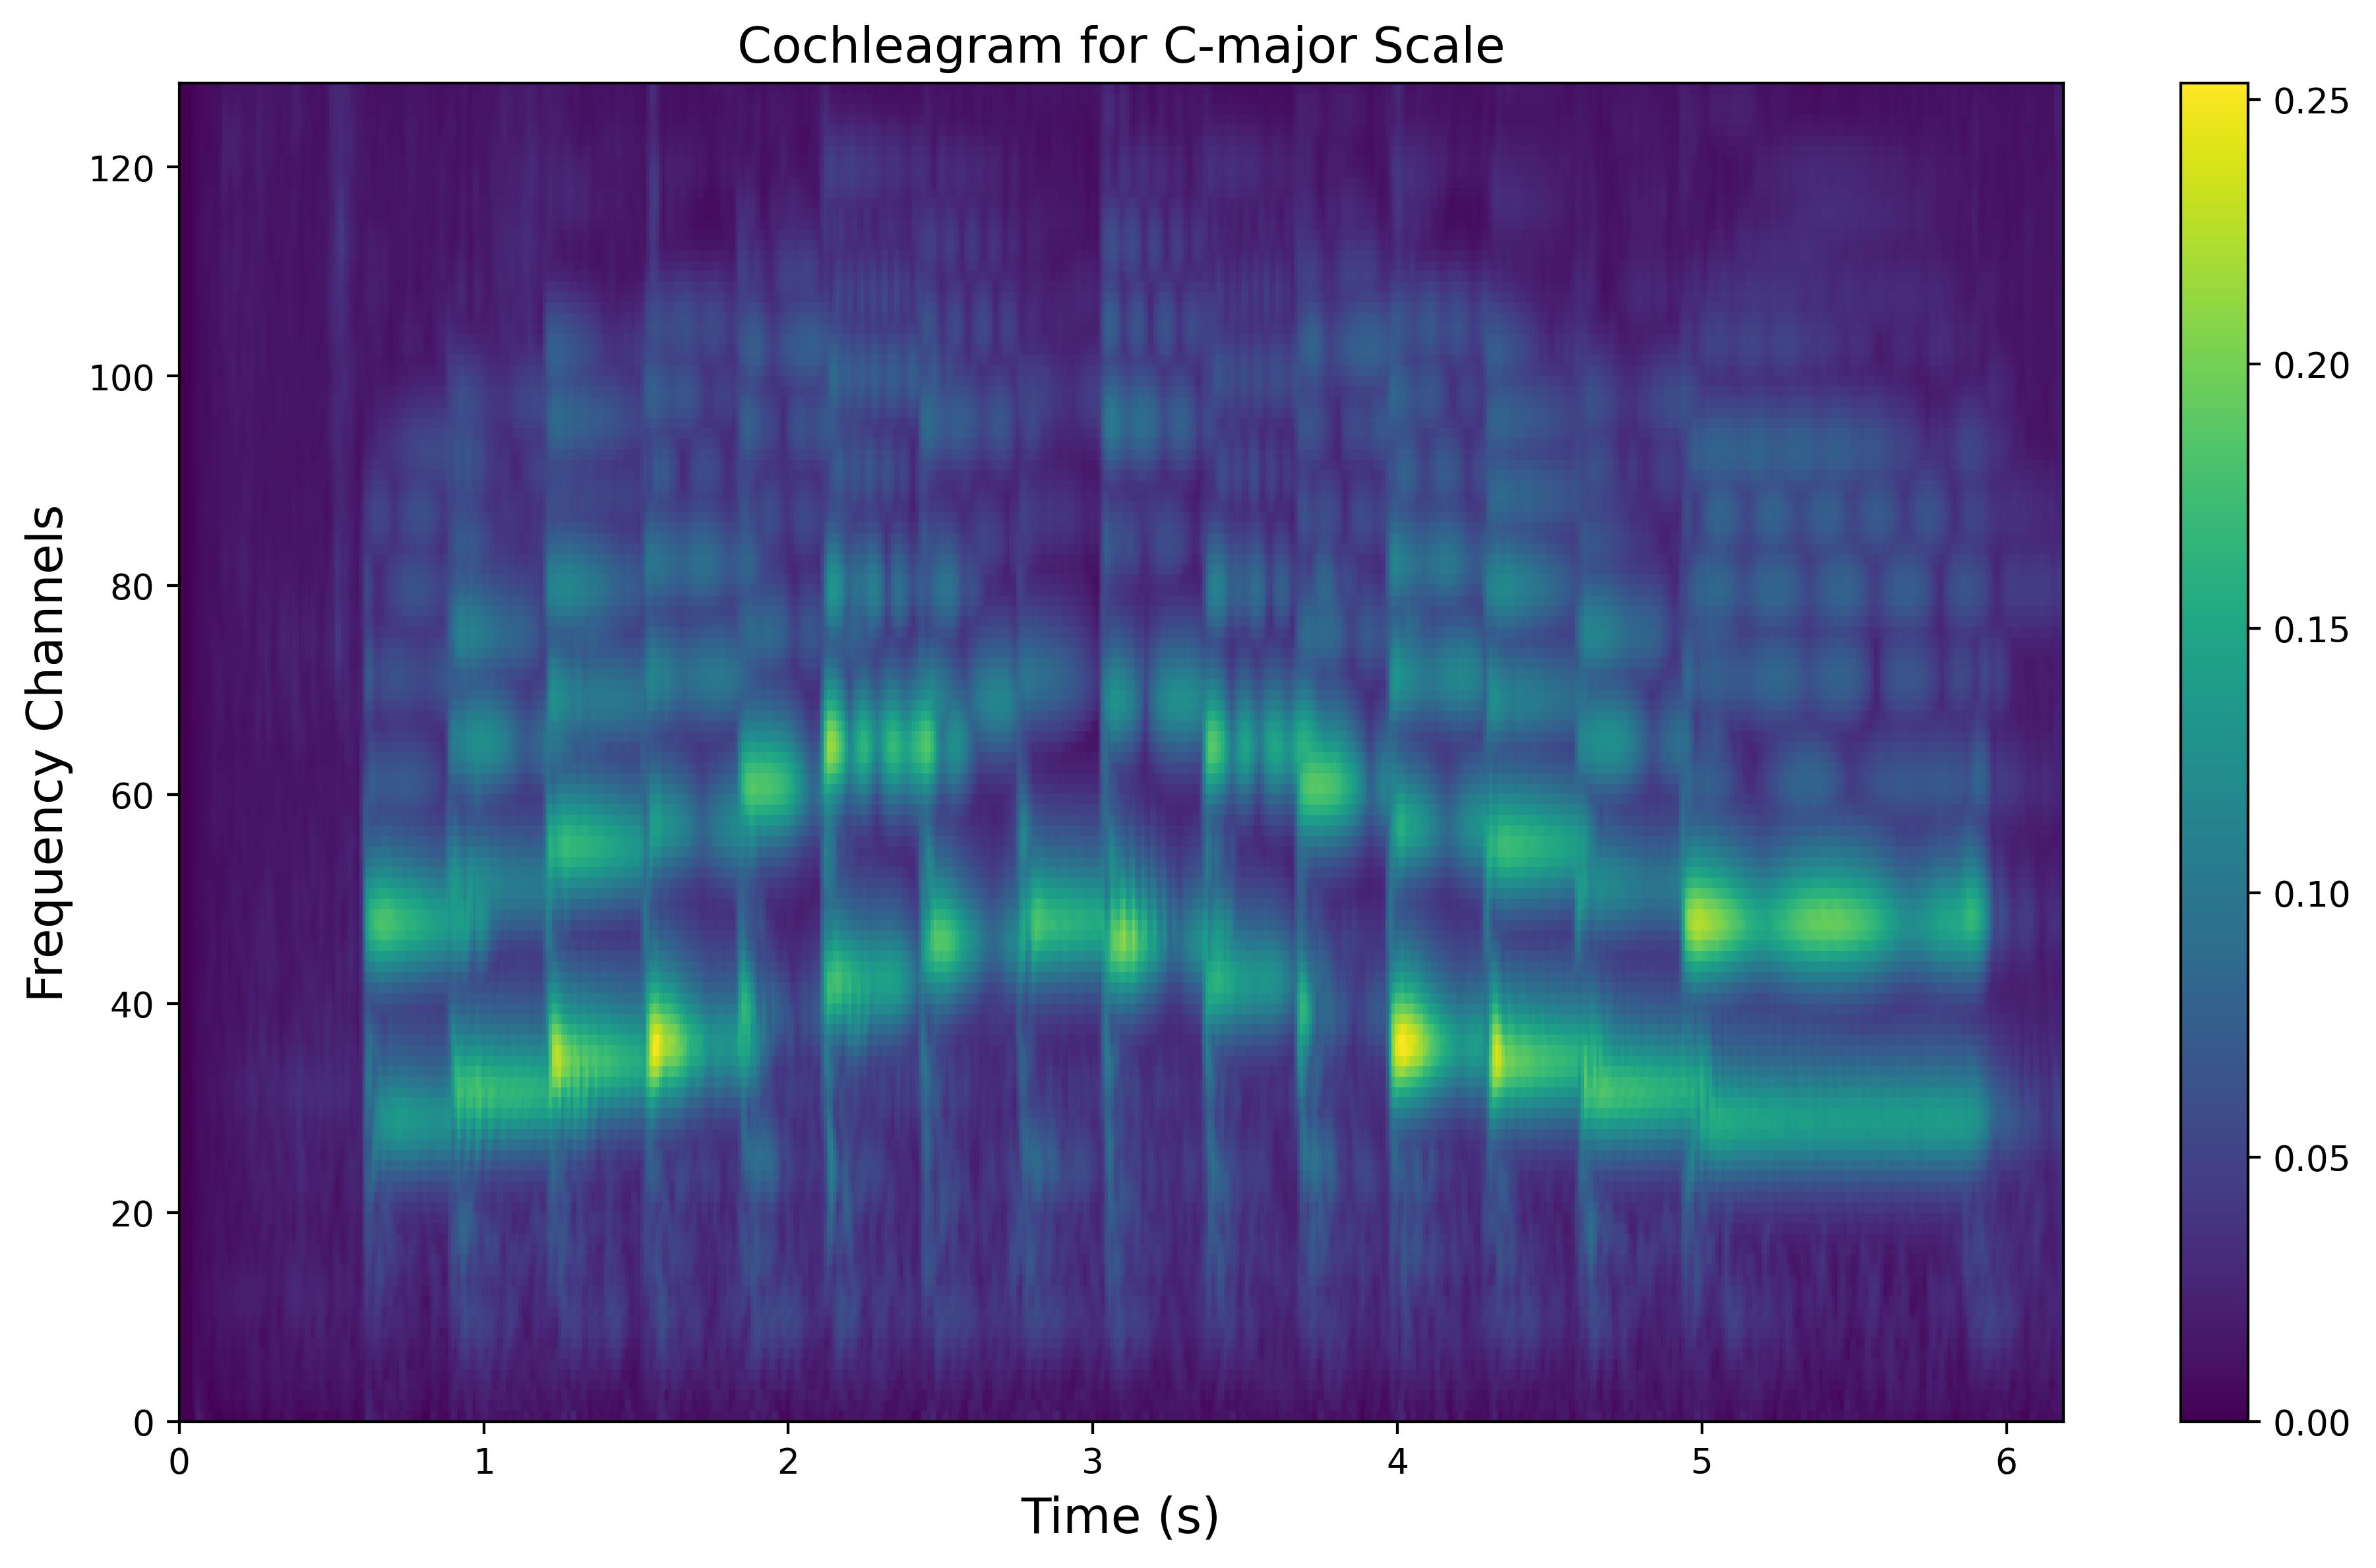
\includegraphics[width=\linewidth]{include/cochleagram_example_C-major}
		\caption{}
	\end{subfigure}%
	\begin{subfigure}{0.5\textwidth}
		\centering
		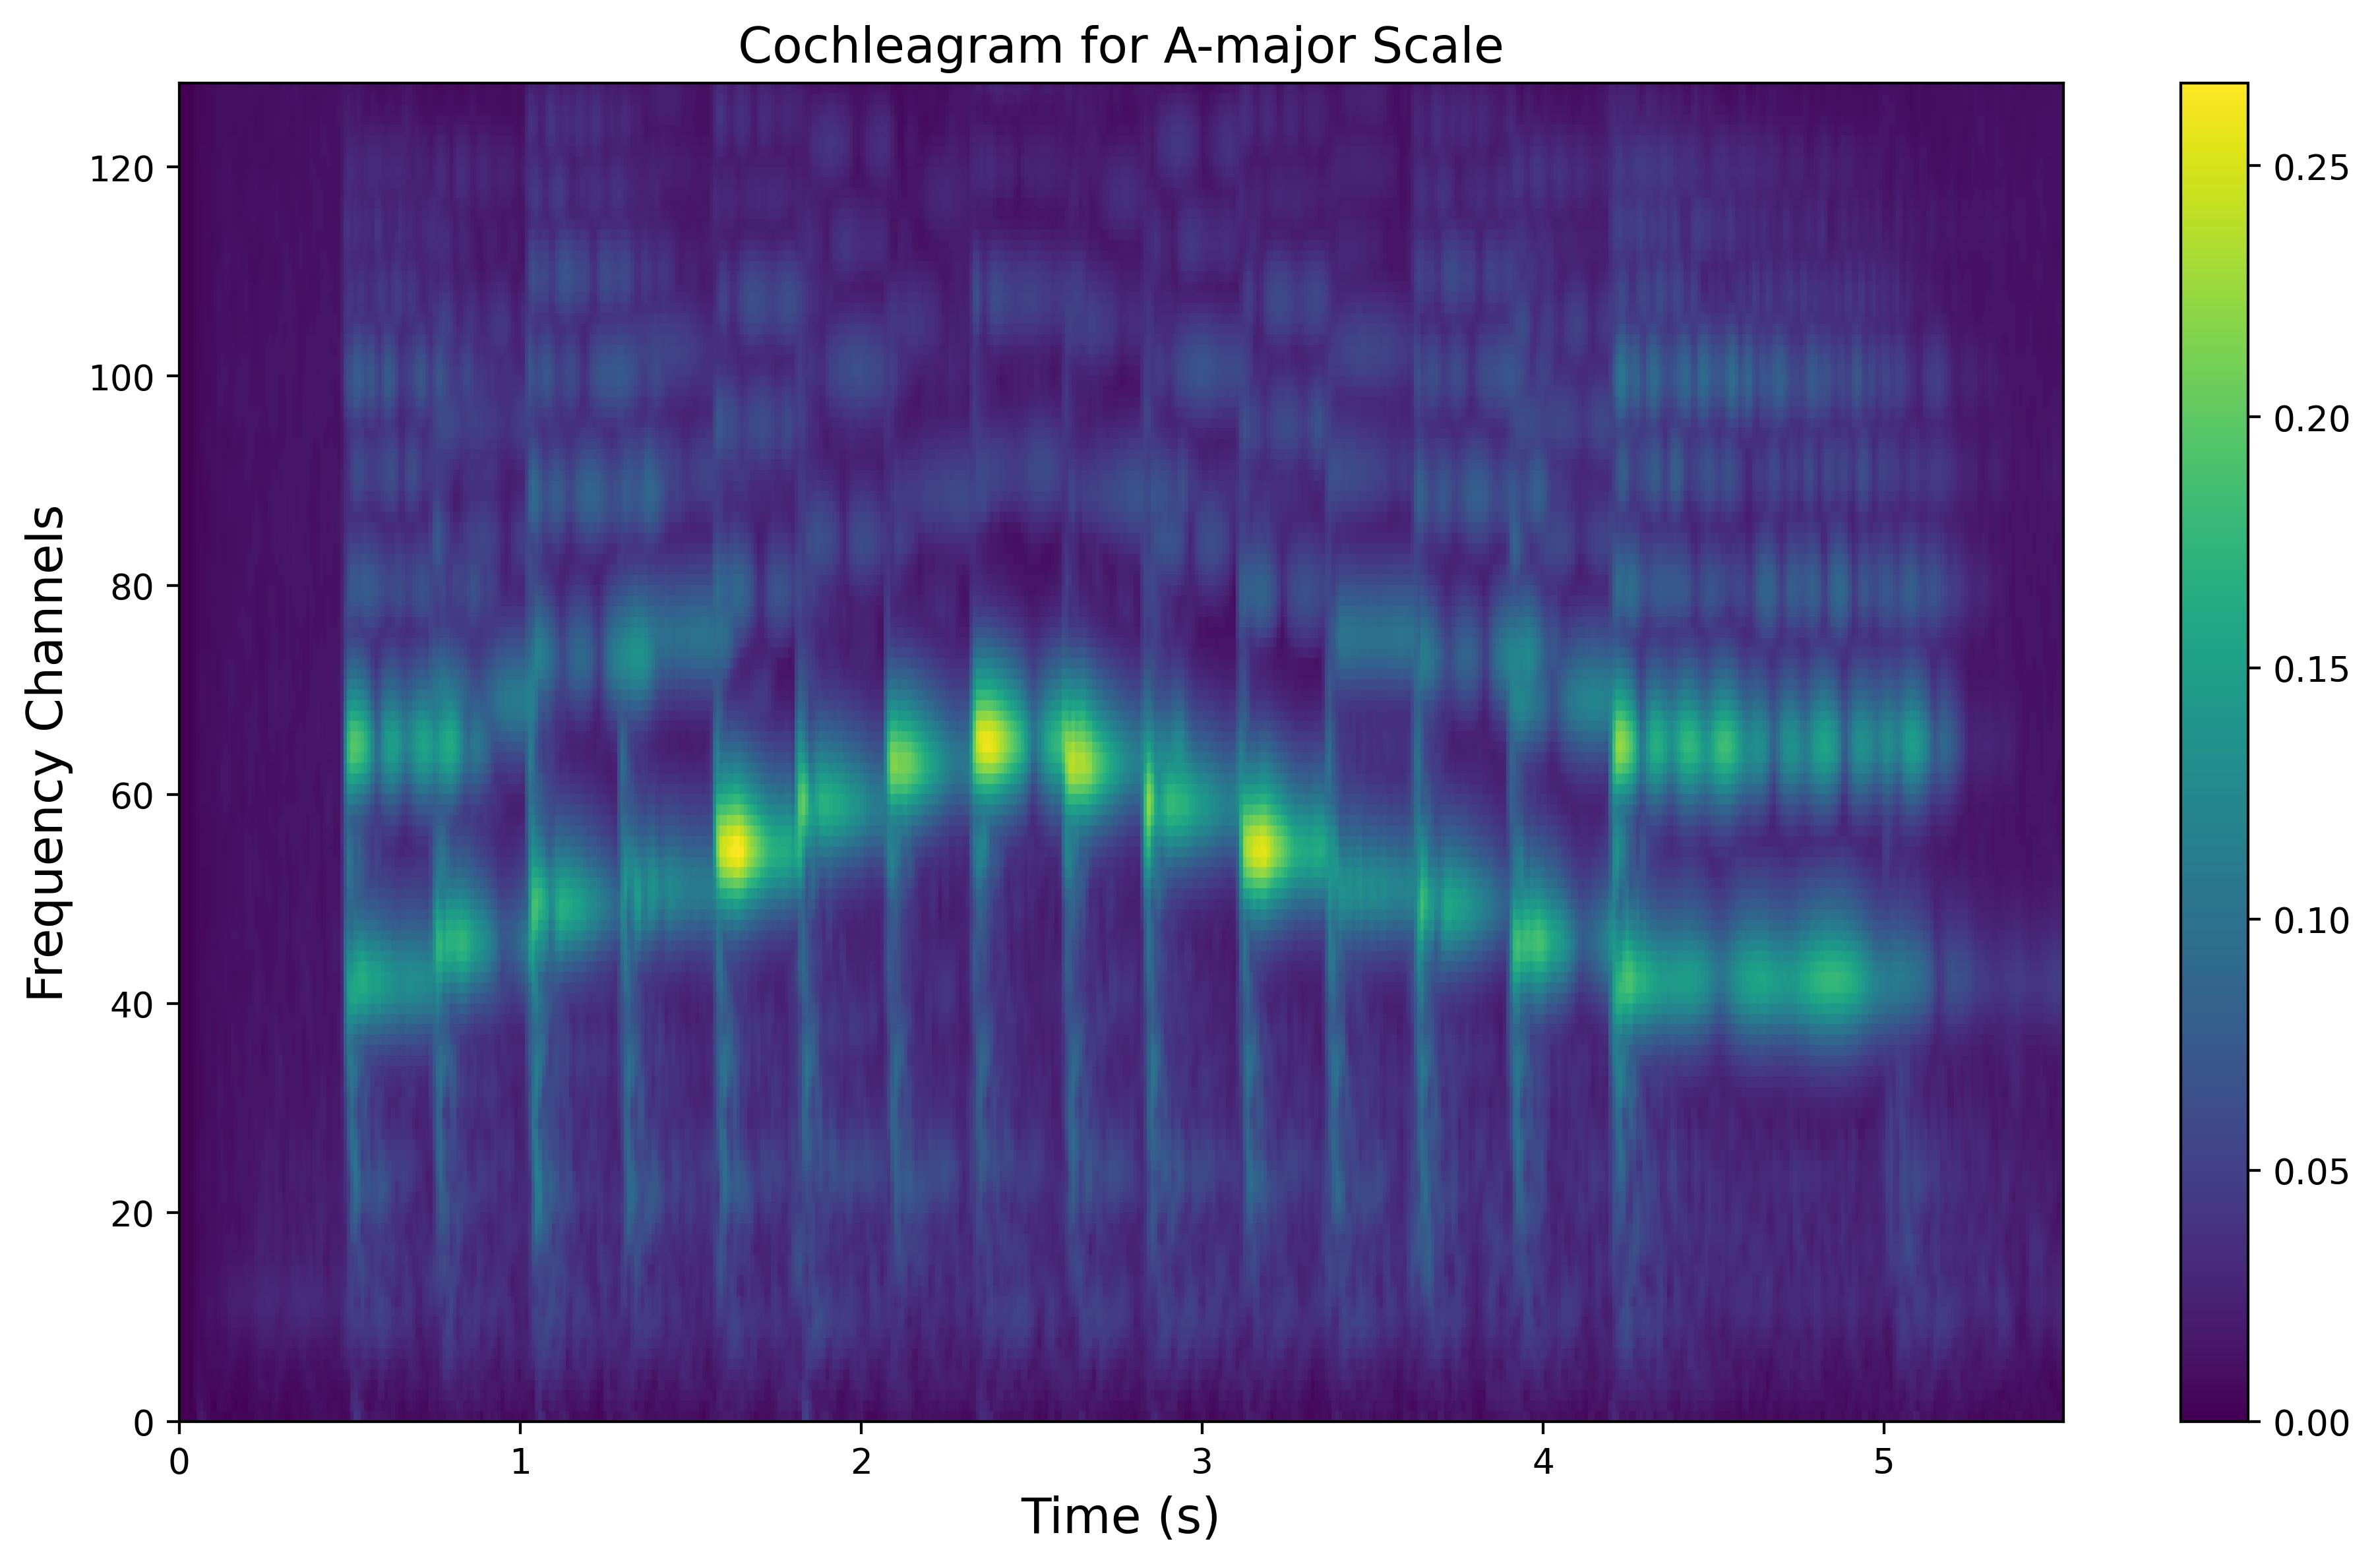
\includegraphics[width=\linewidth]{include/cochleagram_example_A-major}
		\caption{}
	\end{subfigure}
	\caption[Comparison of cochleagrams for C-major and A-major scales]{Cochleagrams for C-major \textbf{(a)} and A-major \textbf{(b)} scales. The ascending and descending note progressions and the note harmonics are clearly visible in both cases, as well as the difference in fundamental frequency between the tones (all notes from A-major scale are higher).}
	\label{img:cochleagram_example}
\end{figure}

After the cochleagram was computed, is was needed to split the output into windows for further processing. A rectangular window of size 20\,ms was used as a default with an overlap of 10\,ms.

\section{Correlogram and Other Features}

For the feature extraction stage described in chapter \ref{subsection:casa_feature_extraction}, a correlogram was implemented using the autocorrelation function implemented in the \textit{statsmodels} package. The provided implementation could compute the ACF similarly as defined in equation \ref{equation:ACF}, however its another variant that uses Fast Fourier Transform was used for higher efficiency. The default number of lags for the autocorrelation function was chosen to be equal to the number of samples in the sampling window, i.\,e.~20\,ms times the samplerate of the input sound (48\,kHz).\\

Thus, the resulting correlogram was a three-dimensional array of floats in $[-1, 1]$ range. The first dimension was time frames, the second was frequency channels and the third was lags for the autocorrelation function.\\

Next, a summary autocorrelation function was computed to help with extracting the fundamental frequencies for separate time frames. The formula was exactly the same as in equation~\ref{equation:SACF}. Also, for demonstration purposes, cross-channel correlation was computed as defined in equation~\ref{equation:CCCF}.\\

Finally, the SACF function was used to estimate the fundamental frequencies of the signals in each time frame. For this step, the "dominant" lags were firstly found, meaning equally spaced lags with the highest sum of SACF values, and then the fundamental frequency was estimated for the current time frame using the distance between two adjacent lags. The default number of "dominant" lags was initially chosen to be 5. The resulting correlogram for time frame 150 is~shown on figure \ref{img:correlogram_example} along with all extracted features.

\begin{figure}[t]
	\centering
	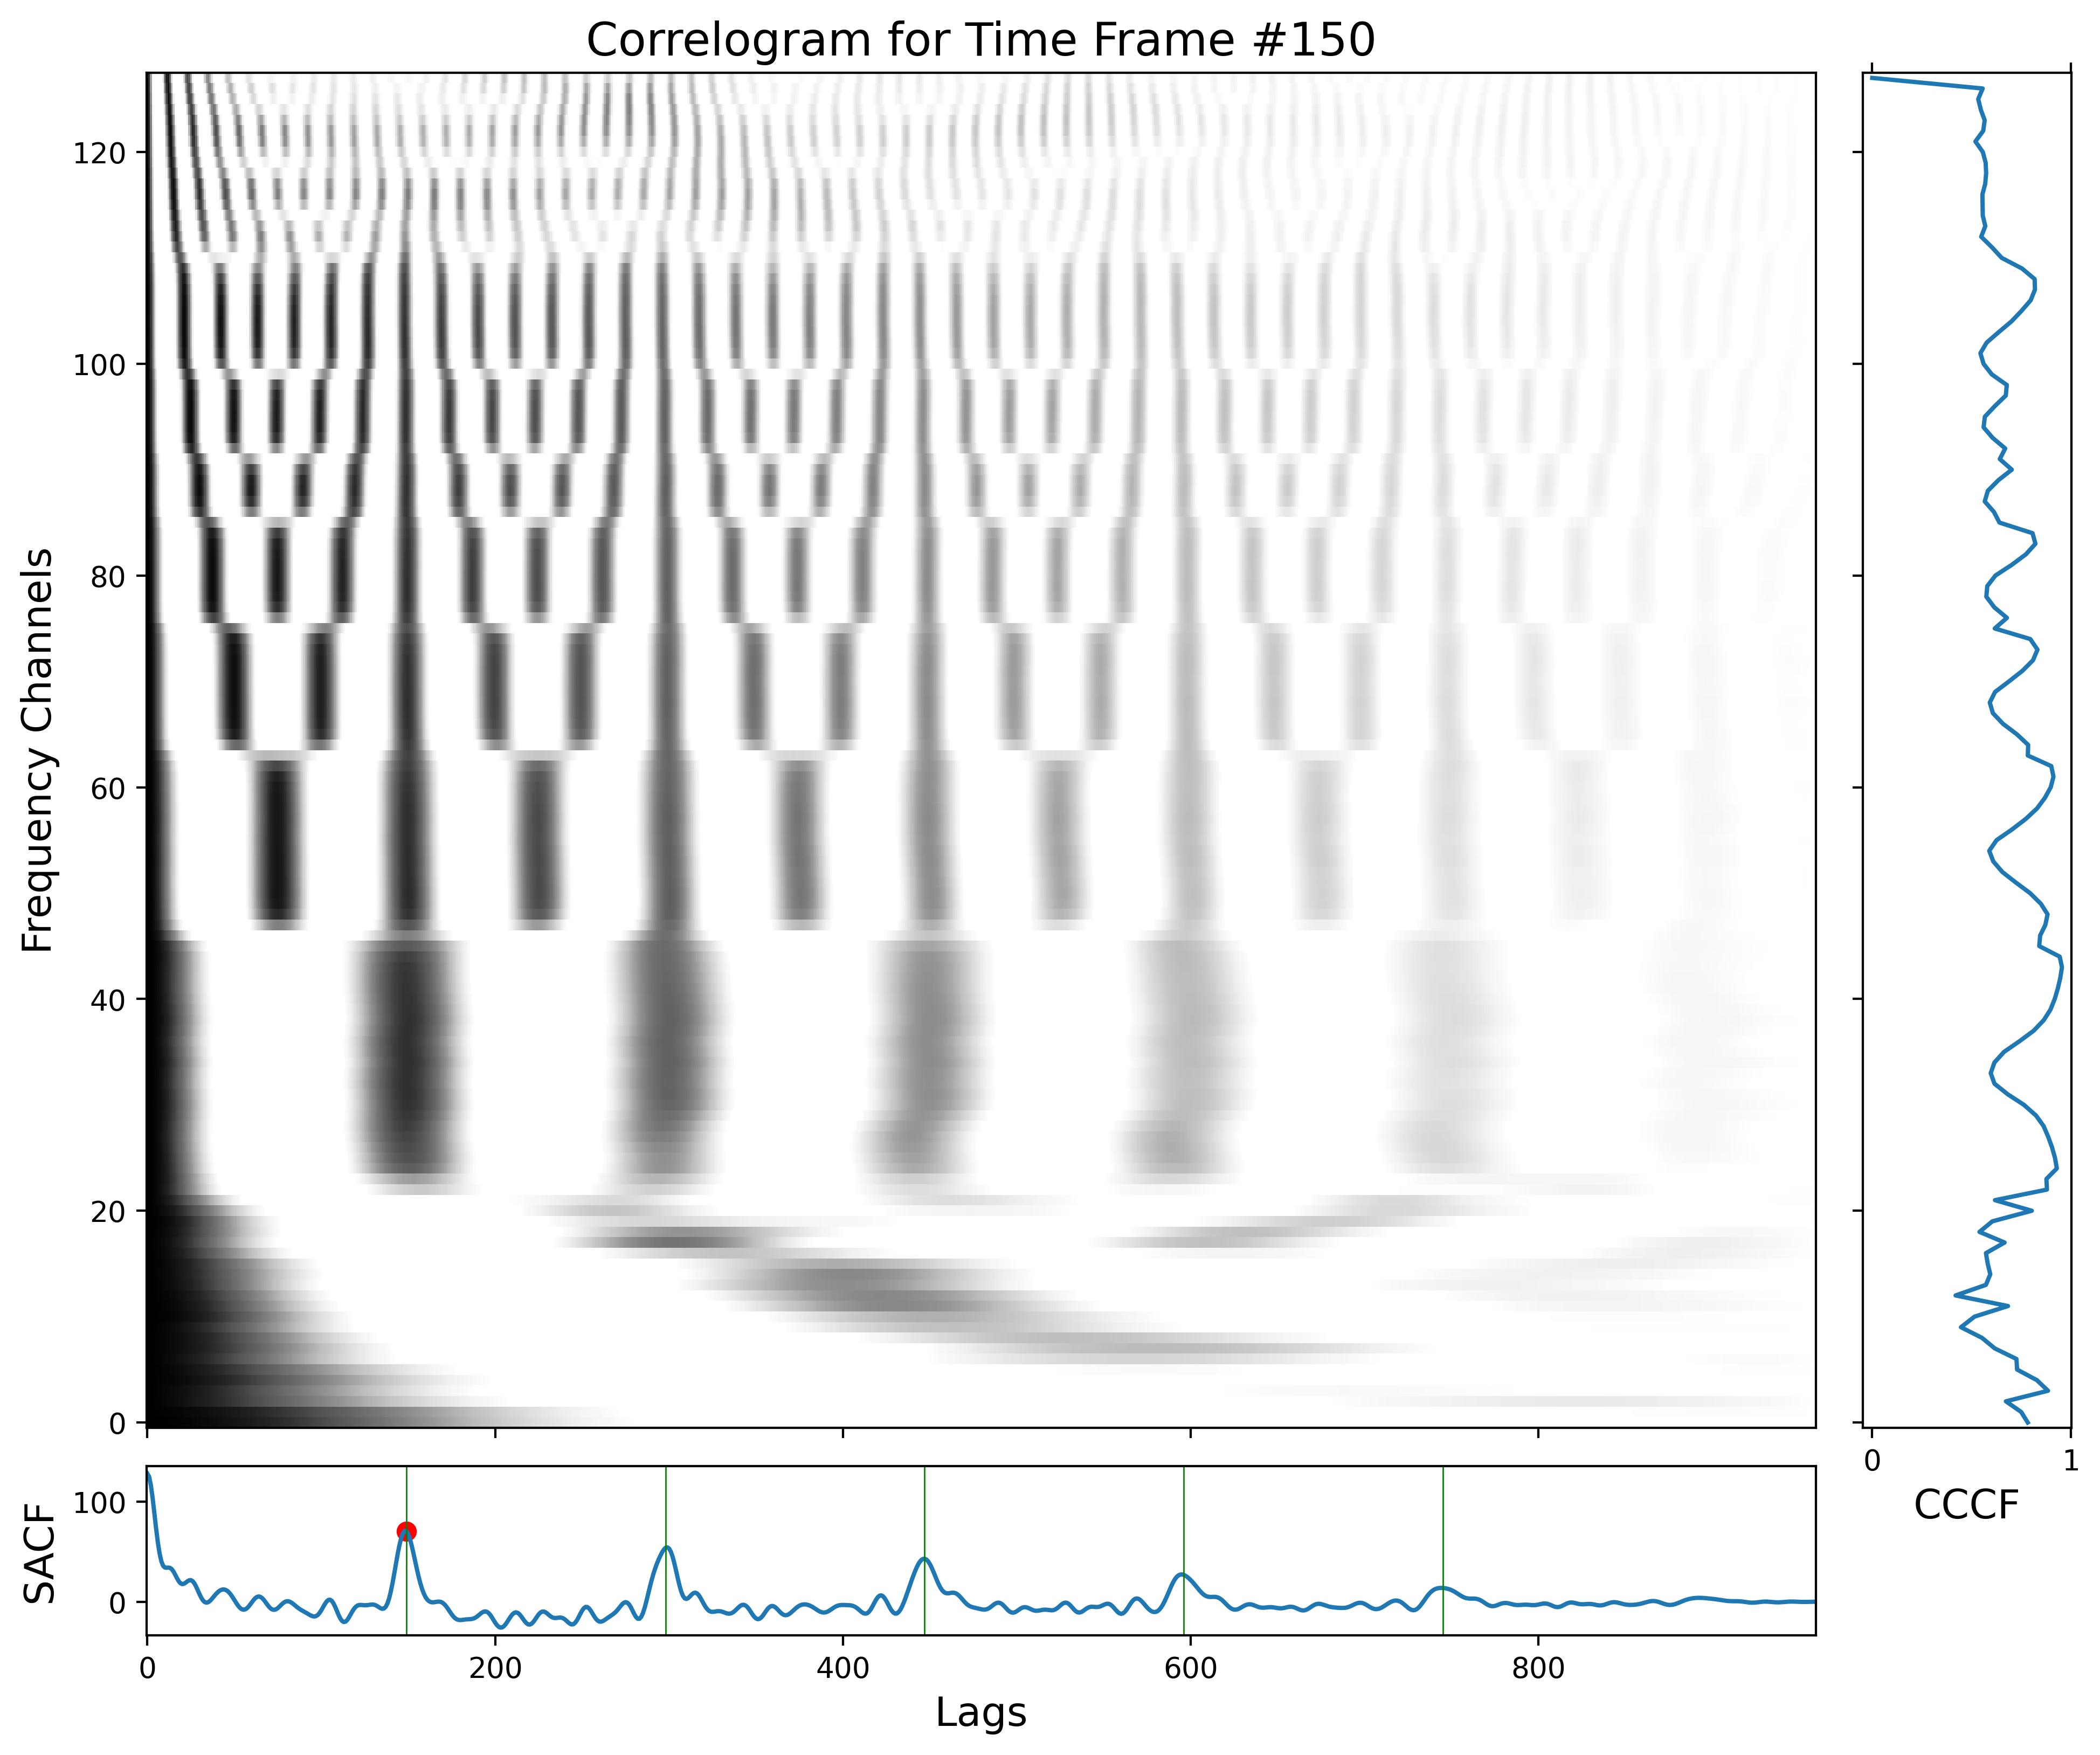
\includegraphics[width=\textwidth]{include/correlogram_example}
	\caption[An example of correlogram and the extracted features for C-major scale]{An example of a correlogram for C-major scale for time frame 150. Note that distinct frequency channels have similar repeating patterns corresponding to the repetitions observed in harmonics. The pattern starts around the frequency channel 40 and repeats twice as fast around channel 60, then three times as fast around channel 70, and so on. Cross-channel correlation is shown on the left panel, and the summary autocorrelation is shown on the bottom panel. Note the peaks on the plot for SACF that emerge when all harmonics become "synchronized". Their corresponding lags are shown as green lines, and the lag corresponding to the fundamental frequency is marked as a red dot.}
	\label{img:correlogram_example}
\end{figure}

\section{Masking}



